\documentclass[a4paper, 10pt]{article}
\usepackage[utf8]{inputenc}
\usepackage{graphicx}
\usepackage{amsmath}

\setlength{\parindent}{0pt}
\setlength{\parskip}{0pt}

\title{Euler spiral}

\begin{document}
\maketitle
An Euler spiral is a curve whose curvature changes linearly with its curve length (the curvature of a circular curve is equal to the reciprocal of the radius). Euler spirals are also commonly referred to as \textit{spiros}, \textit{clothoids}, or \textit{Cornu spirals}. \\

Euler spirals have applications to diffraction computations. They are also widely used as transition curves in railroad engineering/highway engineering for connecting and transitioning the geometry between a tangent and a circular curve. A similar application is also found in photonic integrated circuits. The principle of linear variation of the curvature of the transition curve between a tangent and a circular curve defines the geometry of the Euler spiral: 
\begin{itemize}
		\item Its curvature begins with zero at the straight section (the tangent) and increases linearly with its curve length.
		\item Where the Euler spiral meets the circular curve, its curvature becomes equal to that of the latter.
\end{itemize}
An illustration of the spiral can be seen in figure \ref{fig: spiral}.

\begin{figure}
	\centering
	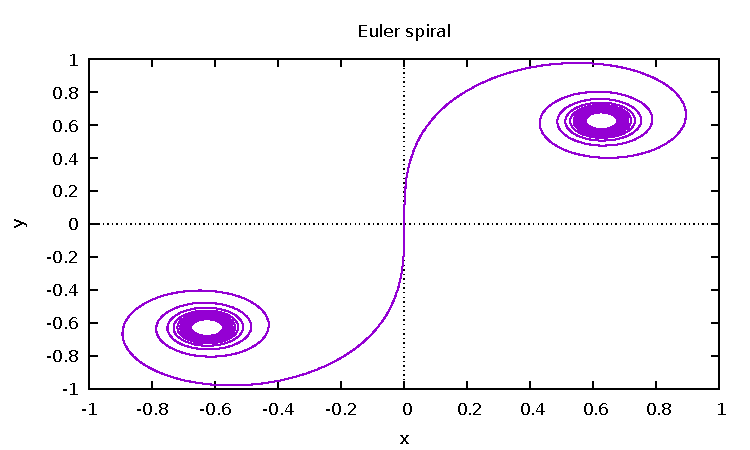
\includegraphics[width=\linewidth]{spiral.pdf}
	\caption{\sl Illustration of the Euler spiral.}
	\label{fig: spiral}
\end{figure}

\section{Applications}
\subsection{Track transition curve}
To travel along a circular path, an object needs to be subject to a centripetal acceleration (e.g.: the moon circles around the earth because of gravity; a car turns its front wheels inward to generate a centripetal force). If a vehicle traveling on a straight path were to suddenly transition to a tangential circular path, it would require centripetal acceleration suddenly switching at the tangent point from zero to the required value; this would be difficult to achieve (think of a driver instantly moving the steering wheel from straight line to turning position, and the car actually doing it), putting mechanical stress on the vehicle's parts, and causing much discomfort (causing jerk). \\

On early railroads this instant application of lateral force was not an issue since low speeds and wide-radius curves were employed (lateral forces on the passengers and the lateral sway was small and tolerable). As speeds of rail vehicles increased over the years, it became obvious that an easement is necessary, so that the centripetal acceleration increases linearly with the traveled distance. Given the expression of centripetal acceleration $V^2/R$, the obvious solution is to provide an easement curve whose curvature, $1/R$, increases linearly with the traveled distance. This geometry is an Euler spiral. \\

Unaware of the solution of the geometry by Leonhard Euler, Rankine cited the cubic curve (a polynomial curve of degree 3), which is an approximation of the Euler spiral for small angular changes in the same way that a parabola is an approximation to a circular curve. \\

Marie Alfred Cornu (and later some civil engineers) also solved the calculus of the Euler spiral independently. Euler spirals are now widely used in rail and highway engineering for providing a transition or an easement between a tangent and a horizontal circular curve.

\subsection{Optics}
The Cornu spiral can be used to describe a diffraction pattern. \cite{ref1}

\section{Formulation}
\subsection{Expansion of Fresnel integral}
If a = 1, which is the case for normalized Euler curve, then the Cartesian coordinates are given by Fresnel integrals (or Euler integrals):
\begin{align*}
	C(L) = \int^z_0 cos(s^2)ds \\
	S(L) = \int^z_0 sin(s^2)ds 
\end{align*}
These two equations were used to generate figure \ref{fig: spiral}.

\begin{thebibliography}{}
	\bibitem{ref1}
	 Eugene Hecht (1998). Optics (3rd ed.). Addison-Wesley. p. 491. ISBN 978-0-201-30425-1.
\end{thebibliography}
\end{document}
